\begin{figure}
  \centering
  \begin{subfigure}[t]{0.26\textwidth}
    \centering
    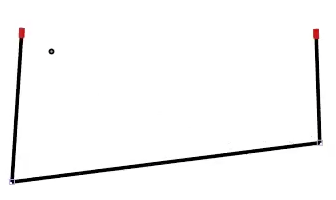
\includegraphics[width=\linewidth]{img/delayed-example-1.png}
    \caption{Initial state.}
    \label{fig:delayed-example-1}
  \end{subfigure}
  \hspace{0.05\linewidth}
  \begin{subfigure}[t]{0.26\textwidth}
    \centering
    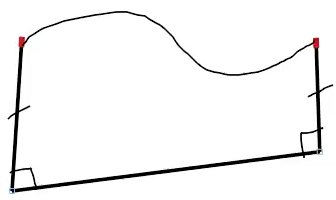
\includegraphics[width=\linewidth]{img/delayed-example-2.png}
    \caption{Five strokes must be recognized.}
    \label{fig:delayed-example-2}
  \end{subfigure}
  \hspace{0.05\linewidth}
  \begin{subfigure}[t]{0.26\textwidth}
    \centering
    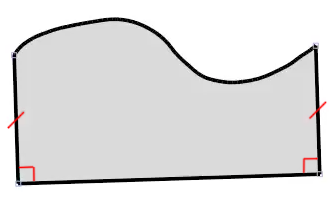
\includegraphics[width=\linewidth]{img/delayed-example-3.png}
    \caption{Input identified as linework and constraints.}
    \label{fig:delayed-example-3}
  \end{subfigure}
  \caption[Delayed Recognizer Example]{Delayed recognizers must be
    able to handle several ink strokes that could compose any number
    of elements. Here the user makes five strokes that must be
    recognized at the same time. This input is identified as four
    distinct items: a Spline, two Right Angles, and a Same Length
    constraint. }
  \label{fig:fig-delayed-example}
\end{figure}
